\documentclass[a4paper, twoside, 11pt]{article}
% It is needed to use this command for automatic compilation in VSCode
% !TEX program = lualatexmk

%% DOCUMENT, PREAMBLE AND MACROS DESIGNED FOR LuaLaTeX %%
\newcommand{\fbar}{\FloatBarrier} % barier for stopping figures from leaking to other subsections, use as \fbar


\usepackage{amsmath} % math package
\usepackage{amssymb} % for miscellaneous mathematical symbols, first usage was for tick symbol in math mode \checkmark
\usepackage{textcomp} % for miscellaneous symbols
\usepackage{graphicx} % enhanced support for graphics
\usepackage{cmap} % mapování znaků - vyhledávání v pdf
% \usepackage[czech]{babel} % CZ
\usepackage[english]{babel} % EN
\usepackage[utf8]{inputenc} % kódování 
\usepackage[T1]{fontenc} % kódování 
\usepackage{multirow} % Multirow table support
\usepackage{float} % Improves the interface for defining floating objects such as figures and tables
\usepackage{wasysym} % for various glyphs, symbols

\usepackage{setspace} % spacing
\onehalfspacing

\usepackage{hyperref}
\hypersetup{
    colorlinks=true, % pokud nechci definovat citecolor=black aby byly odkazy citací černé, tak dám colorlinks=false,%
    bookmarks=true,
    linkcolor=black,
    citecolor=black,
    urlcolor=black,
}

% when using LuaLaTex, defining Times Fonts from your system - it has to be named like this and inserted ttf file in the folder of your tex file
\usepackage{fontspec}
\selectlanguage{czech}
\setmainfont[Ligatures=TeX,BoldFont={Times New Roman Bold}] {Times New Roman}
                                
\setsansfont[Ligatures=TeX,BoldFont={* Bold}]{Times New Roman}
                                      
\setmonofont{CourierPrime-Regular}
 
%\usepackage[italic]{mathastext} % for text in math environment, better looking times then



% for CITATIONS URL to work, it is not needed when you are not using URL label
\usepackage{url}
\usepackage{csquotes}
\usepackage[style=iso-numeric, backend=biber, isbn=true, urldate=iso,seconds=true, date=terse, datezeros=true, language=czech]{biblatex}
\addbibresource{src/bib/zdroje.bib} % BIB resources to import
%\DeclareUrlCommand\url{\def\UrlLeft{<}\def\UrlRight{>} \urlstyle{tt}}
%\usepackage{biblatex}
% END for citations %

% changing bibliography font
\renewcommand*{\bibfont}{\fontspec{Times New Roman}}

\usepackage{comment} % For comments
\usepackage{pdfpages} % for pdf pages
\usepackage{enumerate} % For lists
\usepackage{enumitem} % For Custom Numbering Nested Lists
\setlist[enumerate]{label*=\arabic*.} % setting Number. numbering in lists
\usepackage{tikz} % For vector graphics
\usepackage{circuitikz} % For schemes
\usepackage{pgf} % Post script graphics for tikz

% pouze funguje v PDFLaTeX%
%\usepackage{tgtermes} % na times font, jiný nefunguje s vyhledáváním a copy%

\usepackage{placeins} % for \FloatBarrier command that blocks floating with htbp! go over \FloatBarrier
\usepackage{mathrsfs} % package for math symbols for Laplace, Z transform etc., usage \mathscr{Z}
\usepackage{upgreek} % for upgreek symbols, specified tau \uptau
\usepackage{physics} % for derivations \dd
\usepackage[list=true,listformat=simple]{subcaption}
\usepackage[figurename=Fig.,font=small,labelfont=it,textfont=it]{caption} %for renaming figures instead of renewcommand, small for 11pt default is 10pt as needed in word template
\usepackage[tablename=Tab.,font=small,labelfont=it,
            textfont=it]{caption} % for renaming tables instead of renewcommand
            

%% GLOSSARIES %%
% List of abbreviations and symbols
% Original code author: Jakub Kučera

\usepackage[nonumberlist,nopostdot,section=subsection,numberedsection]{glossaries}
% section = subsection is for glossaries title to appear as a subsection, numberedsection adds the subsec number

\newglossary[slg]{symbolslist}{symbol}{ntn1}{List of symbols}
\newglossary[slg]{abbreviationslist}{abbreviation}{ntn2}{List of abbreviations}

\makeglossaries

% include files with definitions
% PZ definitions
\newglossaryentry{abbreviation:asm}{
                type=abbreviationslist,
                name={ASM},
                description={Asynchronní Motor}
}
\newglossaryentry{abbreviation:pmsynrelm}{
                type=abbreviationslist,
                name={PMSynRelM},
                description={Permanent Magnet Assisted Synchronous Reluctance Motor}
}
\newglossaryentry{abbreviation:synrelm}{
                type=abbreviationslist,
                name={SynRelM},
                description={Synchronous Reluctance Motor}
}
\newglossaryentry{abbreviation:pm}{
                type=abbreviationslist,
                name={PM},
                description={Permanent Magnets}
}
\newglossaryentry{abbreviation:pmsm}{
                type=abbreviationslist,
                name={PMSM},
                description={Permanent Magnet Synchronous Motor}
}
\newglossaryentry{abbreviation:dsp}{
                type=abbreviationslist,
                name={DSP},
                description={Digial Signal Processor}
}
\newglossaryentry{abbreviation:foc}{
                type=abbreviationslist,
                name={FOC},
                description={Field Oriented Control}
}
\newglossaryentry{abbreviation:dtc}{
                type=abbreviationslist,
                name={DTC},
                description={Direct Torque Control}
}
\newglossaryentry{abbreviation:mtpa}{
                type=abbreviationslist,
                name={MTPA},
                description={Maximum Torque Per Ampere}
}
\newglossaryentry{abbreviation:mtpv}{
                type=abbreviationslist,
                name={MTPV},
                description={Maximum Torque Per Voltage}
}
\newglossaryentry{abbreviation:emf}{
                type=abbreviationslist,
                name={EMF},
                description={Electromotive Force}
}
\newglossaryentry{abbreviation:upfc}{
                type=abbreviationslist,
                name={UPFC},
                description={Unity Power Factor Control}
}

\newglossaryentry{abbreviation:pwm}{
                type=abbreviationslist,
                name={PWM},
                description={Pulse Width Modulation}
}


\newglossaryentry{symbol:Pn}{
    type=symbolslist, % glossary
    name=$P_\text{n}$, % jméno v seznamu
    description={jmenovitý výkon}, %popis
    symbol = (W),
    sort=P % seředit podle
}

\newglossaryentry{symbol:Un}{
    type=symbolslist, % glossary
    name=$U_\text{n}$, % jméno v seznamu
    description={jmenovité sdružené napětí}, %popis
    symbol = (V),
    sort=U % seředit podle
}

\newglossaryentry{symbol:fn}{
    type=symbolslist, % glossary
    name=$f_\text{n}$, % jméno v seznamu
    description={jmenovitá napájecí frekvence}, %popis
    symbol = (Hz),
    sort=F% seředit podle
}

\newglossaryentry{symbol:cosphin}{
    type=symbolslist, % glossary
    name=$\cos(\varphi_\text{n})$, % jméno v seznamu
    description={jmenovitý účinník}, %popis
    symbol = (-),
    sort=P% seředit podle
}

\newglossaryentry{symbol:nn}{
    type=symbolslist, % glossary
    name=$n_\text{n}$, % jméno v seznamu
    description={jmenovité otáčky}, %popis
    symbol = (min$^{-1}$),
    sort=P% seředit podle
}


\newglossaryentry{symbol:In}{
    type=symbolslist, % glossary
    name=$I_\text{n}$, % jméno v seznamu
    description={jmenovitý fázový proud stroje}, %popis
    symbol = (A),
    sort=I % seředit podle
}

\newglossaryentry{symbol:u1}{
    type=symbolslist, % glossary
    name=$\underline{u_{1}^{k}}$, % jméno v seznamu
    description={prostorový vektor napětí statorového vinutí}, %popis
    symbol = (V),
    sort=U % seředit podle
}

\newglossaryentry{symbol:u2}{
    type=symbolslist, % glossary
    name=$\underline{u_{2}^{k}}$, % jméno v seznamu
    description={prostorový vektor napětí rotorového vinutí}, %popis
    symbol = (V),
    sort=U % seředit podle
}

\newglossaryentry{symbol:psi1}{
    type=symbolslist, % glossary
    name=$\underline{\psi_1^{k}}$, % jméno v seznamu
    description={prostorový vektor spřaženého magnetického toku statorového vinutí}, %popis
    symbol = (Wb),
    sort=P % seředit podle
}

\newglossaryentry{symbol:psi2}{
    type=symbolslist, % glossary
    name=$\underline{\psi_2^{k}}$, % jméno v seznamu
    description={prostorový vektor spřaženého magnetického toku rotorového vinutí}, %popis
    symbol = (Wb),
    sort=P % seředit podle
}

\newglossaryentry{symbol:r1}{
    type=symbolslist, % glossary
    name=$R_1$, % jméno v seznamu
    description={rezistivita statorového vinutí}, %popis
    symbol = ($\Omega$),
    sort=R % seředit podle
}

\newglossaryentry{symbol:r2}{
    type=symbolslist, % glossary
    name=$R_2$, % jméno v seznamu
    description={rezistivita rotorového vinutí}, %popis
    symbol = ($\Omega$),
    sort=R % seředit podle
}

\newglossaryentry{symbol:i1}{
    type=symbolslist, % glossary
    name=$\underline{i_1^{k}}$, % jméno v seznamu
    description={prostorový vektor proudu statorového vinutí}, %popis
    symbol = (A),
    sort=I % seředit podle
}

\newglossaryentry{symbol:i2}{
    type=symbolslist, % glossary
    name=$\underline{i_2^{k}}$, % jméno v seznamu
    description={prostorový vektor proudu rotorového vinutí}, %popis
    symbol = (A),
    sort=I % seředit podle
}

\newglossaryentry{symbol:omega}{
    type=symbolslist, % glossary
    name=$\omega$, % jméno v seznamu
    description={elektrická úhlová rychlost rotoru}, %popis
    symbol = (s$^{-1}$),
    sort=O % seředit podle
}

\newglossaryentry{symbol:omegas}{
    type=symbolslist, % glossary
    name=$\omega_\text{s}$, % jméno v seznamu
    description={skluzová elektrická úhlová rychlost}, %popis
    symbol = (s$^{-1}$),
    sort=O % seředit podle
}

\newglossaryentry{symbol:omegak}{
    type=symbolslist, % glossary
    name=$\omega_\text{k}$, % jméno v seznamu
    description={obecná elektrická úhlová rychlost}, %popis
    symbol = (s$^{-1}$),
    sort=O % seředit podle
}

\newglossaryentry{symbol:omegamech}{
    type=symbolslist, % glossary
    name=$\Omega$, % jméno v seznamu
    description={mechanická úhlová rychlost}, %popis
    symbol = (s$^{-1}$),
    sort=O % seředit podle
}

\newglossaryentry{symbol:omega1}{
    type=symbolslist, % glossary
    name=$\omega_1$, % jméno v seznamu
    description={elektrická úhlová rychlost točivého magnetického pole}, %popis
    symbol = (s$^{-1}$),
    sort=O % seředit podle
}

\newglossaryentry{symbol:l1}{
    type=symbolslist, % glossary
    name=$L_1$, % jméno v seznamu
    description={indukčnost statorového vinutí}, %popis
    symbol = (H),
    sort=L % seředit podle
}

\newglossaryentry{symbol:j}{
    type=symbolslist, % glossary
    name=$J$, % jméno v seznamu
    description={moment setrvačnosti}, %popis
    symbol = (kg$\cdot$m$^{2}$),
    sort=J % seředit podle
}

\newglossaryentry{symbol:l1sigma}{
    type=symbolslist, % glossary
    name=$L_{1\sigma}$, % jméno v seznamu
    description={rozyptylová indukčnost statorového vinutí}, %popis
    symbol = (H),
    sort=L % seředit podle
}

\newglossaryentry{symbol:l2sigma}{
    type=symbolslist, % glossary
    name=$L_{2\sigma}$, % jméno v seznamu
    description={rozyptylová indukčnost rotorového vinutí}, %popis
    symbol = (H),
    sort=L % seředit podle
}

\newglossaryentry{symbol:lm}{
    type=symbolslist, % glossary
    name=$L_\text{m}$, % jméno v seznamu
    description={magnetizační indukčnost}, %popis
    symbol = (H),
    sort=L % seředit podle
}

\newglossaryentry{symbol:l2}{
    type=symbolslist, % glossary
    name=$L_2$, % jméno v seznamu
    description={indukčnost rotorového vinutí}, %popis
    symbol = (H),
    sort=L % seředit podle
}

\newglossaryentry{symbol:pp}{
    type=symbolslist, % glossary
    name=$p_\text{p}$, % jméno v seznamu
    description={počet polpárů stroje}, %popis
    symbol = (-),
    sort=P % seředit podle
}

\newglossaryentry{symbol:m}{
    type=symbolslist, % glossary
    name=$M$, % jméno v seznamu
    description={vnitřní elektromechanický moment stroje}, %popis
    symbol = (Nm),
    sort=P % seředit podle
}

\newglossaryentry{symbol:mz}{
    type=symbolslist, % glossary
    name=$M$, % jméno v seznamu
    description={zátěžný moment}, %popis
    symbol = (Nm),
    sort=P % seředit podle
}

\newglossaryentry{symbol:slip}{
    type=symbolslist, % glossary
    name=$s$, % jméno v seznamu
    description={skluz}, %popis
    symbol = (-),
    sort=S % seředit podle
}

\newglossaryentry{symbol:u1ef}{
    type=symbolslist, % glossary
    name=$U_1$, % jméno v seznamu
    description={efektivní hodnota fázového napájecího napětí}, %popis
    symbol = (V),
    sort=U % seředit podle
}


\newglossarystyle{myStyleAbbreviations}{
\renewenvironment{theglossary}%
     {\begin{longtable}[l]{llp{\glsdescwidth}p{\glspagelistwidth}}}%
     {\end{longtable}}%
  \renewcommand*{\glossaryheader}{}%
  \renewcommand*{\glsgroupheading}[1]{}%
  \renewcommand{\glossentry}[2]{%
  \glsentryitem{##1} \glstarget{##1}{##2} &
    \textbf{\glossentryname{##1}} &
    \glossentrydesc{##1} &
    ##2\tabularnewline
  }%
  \renewcommand*{\glsgroupskip}{}%  Pokud chci seskupovat podle abeced: \renewcommand*{\glsgroupskip}{ & \\}
}


\newglossarystyle{myStyleSymbols}{
  \renewenvironment{theglossary}%
    {\begin{longtable}[l]{llp{\glsdescwidth}p{\glspagelistwidth}}}%
    {\end{longtable}}%
  \renewcommand*{\glossaryheader}{}%
  \renewcommand*{\glsgroupheading}[1]{}%
  \renewcommand{\glossentry}[2]{%
    \glsentryitem{##1} \glstarget{##1}{\glossentryname{##1}} &
    \glossentrysymbol{##1} &
    \glossentrydesc{##1} &
    ##2\tabularnewline
  }%
  \renewcommand{\subglossentry}[3]{%
     &
     \glssubentryitem{##2}%
     \glossentrysymbol{##2} &
     \glstarget{##2}{\strut}\glossentrydesc{##2} & ##3\tabularnewline
  }%
  \renewcommand*{\glsgroupskip}{%
   }% Pokud chci seskupovat podel abecedy  \ifglsnogroupskip\else & & &\tabularnewline\fi
}
\renewcommand{\glossarypreamble}{\vspace*{-\baselineskip}} % deleting line after glossaries title


%% END OF GLOSSARIES %%

% this works with LuaLaTex and fontspec package %
\DeclareCaptionFont{times}{\fontspec{Times New Roman Italic}}

% labelfont and textfont defined here only works with previous declarecaptionfont times and fontspec
\captionsetup{labelfont=times, textfont=times, labelsep=space}%no separator in captions


%\bibliographystyle{czechiso} %czechiso.bst in folder is needed for this style to work, available at http://www.fit.vutbr.cz/~martinek/latex/czechiso.html%


\usepackage{chngcntr} % for numbered figures with sections
\usepackage{tocloft} % better TOC

%\usepackage{a4wide}%širší a4%
\usepackage[inner=3cm,outer=2cm,top=2.5cm,bottom=2.5cm,footskip=1cm]{geometry}%for propper margins
\usepackage{textcase} % for making text uppercase without caps \MakeTextUppercase
 
 
\usepackage{titlesec} % for spacing text after sections
\usepackage{parskip}[] % for working \parskip
\newcommand{\sectionbreak}{\clearpage} % maybe for SECTIONS on a new page

\usepackage[titletoc]{appendix} % For appendix - přílohy, titletoc is crucial
%\renewcommand{\appendixname}{Příloha}

\setlength{\parindent}{0.5cm} % setting indent of paragraph to 0.5cm
\setlength{\parskip}{0em} % setting parskip to 0 for \titleformat to work properly with parskip package

\usepackage{colortbl} % for colored cells in tables
\usepackage{xcolor} % for color definitions

%% COLOR DEFINITIONS %%
\definecolor{ctublue}{HTML}{0065BD} % defining ctu color
\definecolor{ctugreen}{HTML}{A2AD00}
\definecolor{ctured}{HTML}{C60C30}
\definecolor{ctuyellow}{HTML}{F0AB00}
\definecolor{ctugreenyblue}{HTML}{00B2A9}
\definecolor{ctulightblue}{HTML}{6AADE4}
\definecolor{ctuorange}{HTML}{E05206}
\definecolor{lightgray}{HTML}{D1D5DB}
\definecolor{codeblue}{HTML}{D9E2F3}
\definecolor{codegreen}{rgb}{0,0.6,0}
\definecolor{codegray}{rgb}{0.5,0.5,0.5}
\definecolor{codepurple}{rgb}{0.58,0,0.82}
\definecolor{backcolour}{rgb}{0.95,0.95,0.92}

% defining spacing of titles
\titlespacing*{\section}{0em}{1em}{-\parskip} % spacing text after sections from titlesec package
\titlespacing*{\subsection}{0em}{1em}{-\parskip} % spacing text after sections from titlesec package
\titlespacing*{\subsubsection}{0em}{1em}{-\parskip} % spacing text after sections from titlesec package

% defining style for titles
% when you want section/sub/subsub to be black, delete \color{ctublue}
\titleformat{\section}{\color{ctublue}\fontspec{Times New Roman}\fontsize{15}{15}\bfseries}{\thesection}{2.1em}{}%defining title sizes by word template
\titleformat{\subsection}{\color{ctublue}\fontspec{Times New Roman}\fontsize{14}{14}\bfseries}{\thesubsection}{1.53em}{}%defining title sizes by word template
\titleformat{\subsubsection}{\color{ctublue}\fontspec{Times New Roman}\fontsize{13}{13}\bfseries}{\thesubsubsection}{1em}{}%defining title sizes by word template


\usepackage{ctable} % imports xtable with booktabs
\usepackage{multicol} % for multicolumn feature in tables

\usepackage{listings} % for code environments - \begin{lstlisting}

% solving problems with ) literal to be coded in lstlisting as it should be
\makeatletter
\patchcmd{\lsthk@SelectCharTable}{)}{`}{}{} 
\makeatother 

\lstdefinestyle{zakopal}{
    backgroundcolor=\color{codeblue},   
    commentstyle=\color{codegray},
    keywordstyle=\color{ctured},
    numberstyle=\tiny\color{codegray},
    stringstyle=\color{ctuorange},
    basicstyle=\ttfamily\small,
    breakatwhitespace=false,         
    breaklines=true,                 
    captionpos=b,                    
    keepspaces=true,                 
    numbers=left,                    
    numbersep=5pt,                  
    showspaces=false,                
    showstringspaces=false,
    showtabs=false,                  
    tabsize=2
}
\lstset{style=zakopal}
\renewcommand{\lstlistingname}{Code}% renaming Listing -> Kód 
\renewcommand{\lstlistlistingname}{List of codes}% renaming List of Listings -> Seznam kódů

\lstdefinelanguage{SCL}
{morekeywords={FUNCTION_BLOCK,BEGIN,NOT,END_FUNCTION_BLOCK,FUNCTION,VOID,VAR_INPUT,END_VAR,VAR_IN_OUT,IF,
THEN,END_IF,END_FUNCTION,BOOL,FALSE,TRUE},
sensitive=false,
morecomment=[l]{//},
morestring=[b]",
literate={;}{{\textcolor{ctuorange}{;}}}{1}
{:}{{\textcolor{ctuorange}{:}}}{1}
{)}{{\textcolor{ctuorange}{)}}}{1}
{(}{{\textcolor{ctuorange}{(}}}{1}
{=}{{\textcolor{ctuorange}{=}}}{1}
{,}{{\textcolor{ctuorange}{,}}}{1},} %basic SCL language for siemens defined%

\lstdefinelanguage{xdc}
{morekeywords={set_property, current_design, get_ports},
sensitive=false,
morecomment=[l]{\#}} %basic xdc file in Vivado syntax highlighting%

\lstdefinelanguage{xsct}
{morekeywords={xsct, hsi, open_hw_design, -createdts, -hw, -zocl, -platform-name, -overlay, -compile, -out, exit, -git-branch},
alsoletter={-},
sensitive=false,
morecomment=[l]{\#}} %xsct (Xilinx Software Command-Line Tools)%


\lstdefinelanguage{Text}
{morekeywords={},
alsoletter={-},
sensitive=false,
morecomment=[l]{//},
morecomment=[l]{\#}} %basic text%

\lstdefinelanguage{devicetree}
{morekeywords={chosen, bootargs, stdout-path, compatible, status},
alsoletter={-},
stringstyle=\color{ctuorange},
moredelim=[s][\color{ctuorange}]{"}{"},
sensitive=false,
morecomment=[l]{\#},
literate={\{}{{\textcolor{ctured}{\{}}}{1}
{\}}{{\textcolor{ctured}{\}}}}{1}
} %devicetree%

\lstdefinelanguage{json}
{morekeywords={},
upquote=true,
morestring=[b]",
stringstyle=\color{ctuorange},
moredelim=[s][\color{ctuorange}]{"}{"},
sensitive=false,
morecomment=[l]{\#},
literate=
     *{0}{{{\color{ctured}0}}}{1}
      {1}{{{\color{ctured}1}}}{1}
      {2}{{{\color{ctured}2}}}{1}
      {3}{{{\color{ctured}3}}}{1}
      {4}{{{\color{ctured}4}}}{1}
      {5}{{{\color{ctured}5}}}{1}
      {6}{{{\color{ctured}6}}}{1}
      {7}{{{\color{ctured}7}}}{1}
      {8}{{{\color{ctured}8}}}{1}
      {9}{{{\color{ctured}9}}}{1}
      {\{}{{{\color{ctured}{\{}}}}{1}
      {\}}{{{\color{ctured}{\}}}}}{1}
      {[}{{{\color{ctured}{[}}}}{1}
      {]}{{{\color{ctured}{]}}}}{1},
} %json%

\lstdefinelanguage{pseudocode}
{morekeywords={if, else, positive, negative, edge, end},
alsoletter={-},
stringstyle=\color{ctuorange},
moredelim=[s][\color{ctuorange}]{"}{"},
sensitive=false,
morecomment=[l]{\//},
literate={\{}{{\textcolor{ctured}{\{}}}{1}
{\}}{{\textcolor{ctured}{\}}}}{1}
{(}{{{\color{ctured}{(}}}}{1}
{)}{{{\color{ctured}{)}}}}{1}
} %devicetree%


%%change in previous commands 2.1 em , 1.53em and 1em to 1em to be easy indented not the same
\begin{document}
\fontspec{Times New Roman}

\counterwithin{figure}{section}%changing counter of figure, at each section the numbering resets
\counterwithin{table}{section}%changing counter of table, at each section the numbering resets
\counterwithin{equation}{section}%changing counter of equation, at each section the numbering resets

\counterwithin{lstlisting}{section}%counter of lstlist - codes, reseting at each section%


\renewcommand{\thefigure}{\thesection~-~\arabic{figure}}%defining style of countering
\renewcommand{\thetable}{\thesection~-~\arabic{table}}
\renewcommand{\theequation}{\thesection~-~\arabic{equation}}
\renewcommand{\thelstlisting}{\thesection~-~\arabic{lstlisting}}%delfining style for lstlisting codes, needs to be after begin document as previous renewcommand%

\renewcommand*{\cftsecdotsep}{1}  % use dots in the section entries and their step
\renewcommand*{\cftsubsecdotsep}{1}
\renewcommand*{\cftsubsubsecdotsep}{1}
\renewcommand*{\cftsecnumwidth}{4em} % increase space for Roman numerals
\renewcommand*{\cftsubsecnumwidth}{4em} %numbering width
\renewcommand*{\cftsubsubsecnumwidth}{4em} %numbering width
\renewcommand*{\cftsubsubsecindent}{0em}%no indent for subsubsection
\renewcommand*{\cftsubsecindent}{0em}%no indent for subsection
\renewcommand*{\cftsecindent}{0em}%no indent for subsection



\renewcommand*{\cftfigdotsep}{1}  % use dots in the figure entries and their step
\renewcommand*{\cftfignumwidth}{4em}
\renewcommand*{\cftfigindent}{0em}

\renewcommand*{\cfttabdotsep}{1}  % use dots in the figure entries and their step
\renewcommand*{\cfttabnumwidth}{4em}
\renewcommand*{\cfttabindent}{0em}

\renewcommand{\cftsecfont}{\fontspec{Times New Roman}\large \bfseries}
\renewcommand{\cftsubsecfont}{\fontspec{Times New Roman}}
\renewcommand{\cftsubsubsecfont}{\fontspec{Times New Roman}}

\renewcommand{\cftfigfont}{\fontspec{Times New Roman}}
\renewcommand{\cfttabfont}{\fontspec{Times New Roman}}

\renewcommand*\contentsname{\textcolor{ctublue}{\MakeTextUppercase{\fontspec{Times New Roman}Table of Contents}}}
\renewcommand{\listtablename}{{\fontspec{Times New Roman}\textcolor{ctublue}{\MakeTextUppercase{{List of tables}}}}}
\renewcommand{\listfigurename}{{\fontspec{Times New Roman}\textcolor{ctublue}{\MakeTextUppercase{{List of figures}}}}}


%% TITLE PAGE %%
\setcounter{figure}{0}

\begin{titlepage}
	\begin{center}

\begin{figure}[H]
	\begin{center}
		
\includegraphics[scale=1]{src/misc/symbol_cvut_konturova_verze.pdf}
	\end{center}
\end{figure}
	{\Large{\textbf{CZECH TECHNICAL UNIVERSITY IN PRAGUE}}}\\
	{\textbf{Faculty of Electrical Engineering}}\\
	{\textbf{Department of Electric Drives and Traction}}
	
	\vspace{3cm}
	
	
	{\Large\textbf{Title}}
	
	\vspace{1cm}
	
	%{\Large\textbf{Possibilities of Using SoC Platform Processors for Controlling Electric Drives}}
	
	%\vspace{2cm}
	
	Subtitle\\
	
	\end{center}
	
	\vspace{3cm}
	
	%\noindent Studijní program: Elektrotechnika, Energetika a Management\\
	%\noindent Studijní obor: Elektrické pohony
	
	\vspace{0.5cm}
	%\noindent Vedoucí práce: doc. Ing. Jan Bauer, Ph.D.
	
	\vfill
	
\begin{center}

	\large{\textbf{Petr Zakopal}}\\
	\large{\textbf{Prague 2023}}
	\end{center}
\end{titlepage}


\newpage
\pagenumbering{gobble} %disabling page numbering

\newpage


%%ZADÁNÍ PRÁCE
%verze pro TISK - jen s NEW PAGE


%ONLINE VERZE - se zadáním BEZ PODPISŮ
% online verze - odkomentovat následující dva řádky
%\null\newpage
%\includepdf[]{src/docs/zadani_bez_podpisu.pdf}

%\newpage
%\cleardoublepage
\null\newpage

\pagenumbering{Roman}
\setcounter{page}{2}%%3 NUTNO řešit dle zadání etc.

%% PROHLASENI A PODEKOVANI %%
%  \noindent \textcolor{ctublue}{{\Large{\textbf{\MakeTextUppercase{Prohlášení}}}}}\\
 			Prohlašuji, že jsem předloženou práci vypracoval samostatně a že jsem uvedl veškeré použité informační zdroje v~souladu s~Metodickým pokynem o~dodržování etických principů při přípravě vysokoškolských závěrečných prací.\\
 		\vspace{1.5cm}
		
	

 	\noindent	V~Praze dne \rule{3.5cm}{0.4pt} \hspace{6.6cm}  \rule{4cm}{0.4pt}
	
 	\hspace{12.65cm}Petr Zakopal


 		\vspace{14cm}
		
 	\noindent	\textcolor{ctublue}{{\Large{\textbf{\MakeTextUppercase{Poděkování}}}}}\\
 	Tímto bych rád poděkoval vedoucímu této práce doc. Ing. Janu Bauerovi, Ph.D. za skvělé vedení práce a cenné rady při jejím vytváření. Dále bych rád poděkoval všem, kteří mě v~mém dosavadním studiu podporovali.
	


%%ABSTRAKT%%
%  \newpage
 %\addcontentsline{toc}{section}{3\quad Abstrakt a klíčová slova}%Added citations to TOC%
 %\begin{comment}
 \begin{minipage}[t]{7.37cm}
 		\raggedright
 	\textcolor{ctublue}{\Large{\textbf{\MakeTextUppercase{Abstrakt}}}}\\
    Textík.
	
 \end{minipage}%
 \hfill% --- important, otherwise it wont be so nice
 \begin{minipage}[t]{7.37cm}
 		\textcolor{ctublue}{\Large{\textbf{\MakeTextUppercase{Abstract}}}}\\
	Textík v aj.	
 \end{minipage}
% %\end{comment}
% 	%\textcolor{ctublue}{\Large{\textbf{\MakeTextUppercase{Abstrakt}}}}\\

% 	%\textcolor{ctublue}{\Large{\textbf{\MakeTextUppercase{Abstract}}}}\\

% \newpage



%% TABLE OF CONTENTS %%
\tableofcontents
\newpage%
\flushbottom % vyčištění stránky
\newpage
\vspace{0pt}

%% LIST OF FIGURES %%
\listoffigures % seznam obrázků
\flushbottom % vyčištění stránky
\newpage

%% LIST OF TABLES %%
\listoftables
\flushbottom

\newpage


%% BLANK PAGE AFTER TOC, TOF, TOT %%
\pagenumbering{gobble}
\null\newpage

% setting the page numbering to start from 1, where the main text starts
\setcounter{page}{1}
\pagenumbering{arabic}

\section{Introduction}
\gls{symbol:Pn} \gls{abbreviation:asm}

\section{Design}
The Permanent Magnet assisted synchronous reluctance motor (\gls{abbreviation:pmsynrelm}) is widely used for it's significant advantages of small size, low loss, high efficiency, better performance than plain synchronous reluctance motors \gls{abbreviation:synrelm} and wide constant power to speed range. \cite{xinmin-design-of-permanent-magnet-assisted-synch-rel-m-with-low-torque-ripple,huynh-design-and-analysis-of-perm-as-synch-rel-m}
    \subsection{Stator and Rotor}
        There are many solutions on how to connect the stator winding. Research has been carried out for standard Delta or Start winding, but to increase the torque for same stator current the combined Start-Delta winding was proposed. The first research has been caried out for standard \gls{abbreviation:synrelm} in \cite{ibrahim-an-improved-torque-density-synchronous-reluctance-machine-with-a-combined-star-delta-winding-layout} and then extended to \gls{abbreviation:pmsynrelm} prototypes in \cite{ibrahim-permanent-magnet-assisted-synchronous-reluctance-motor-employing-a-hybrid-star-delta-winding-for-high-speed-applicaitons}. The main idea of the hybrid Delta-Star connection is to split the standard phase wiring into two parts. The one part is for the Delta connection, the other for Star connection. Then the coils of wiring are connnected to series. Motors utilizing hybrid stator winding with \gls{abbreviation:pm}s inserted in the rotor flux bariers exhibit constant power factor over 0.9

        \begin{figure}[htbp!]
            \centering
            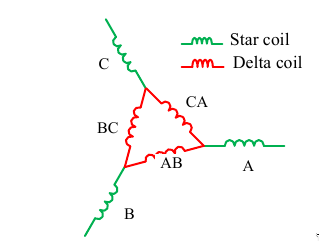
\includegraphics[width=0.5\textwidth]{src/png/hybrid-star-delta-wiring.png}
            \caption{Hybrid Star-Delta wiring of \gls{abbreviation:pmsynrelm}. {\textcolor{ctured}{CHANGE THIS IMAGE FOR YOUR OWN, IT IS FROM \cite{ibrahim-permanent-magnet-assisted-synchronous-reluctance-motor-employing-a-hybrid-star-delta-winding-for-high-speed-applicaitons}}}}
            \label{fig:hybrid-star-delta-wiring}
        \end{figure}

        In \cite{ibrahim-permanent-magnet-assisted-synchronous-reluctance-motor-employing-a-hybrid-star-delta-winding-for-high-speed-applicaitons} the authors manufactured proposed four prototypes. The prototypes consist of two stators, with either conventional star winding or hybrid star-delta winding, and two rotors, with ferrite permanent magnets or without. Maxwell transient simulations were carried out on the four prototypes, which were then manufactured and experiment using the simulation results was conducted.
\par
    According to \cite{ibrahim-permanent-magnet-assisted-synchronous-reluctance-motor-employing-a-hybrid-star-delta-winding-for-high-speed-applicaitons} the researches state, that when using the hybrid stator winding connection, the efficiency increase is rather low compared to efficiency increase when comparing \gls{abbreviation:synrelm} with and without \gls{abbreviation:pm}s.\par
    The design of the \gls{abbreviation:pmsynrelm} rotor with \gls{abbreviation:pm} oriented solely in the $q$-axis is depicted in the figure \ref{fig:pmsynrelm-rotor-magnets-q-axis}.
    
    \begin{figure}[htbp!]
            \centering
            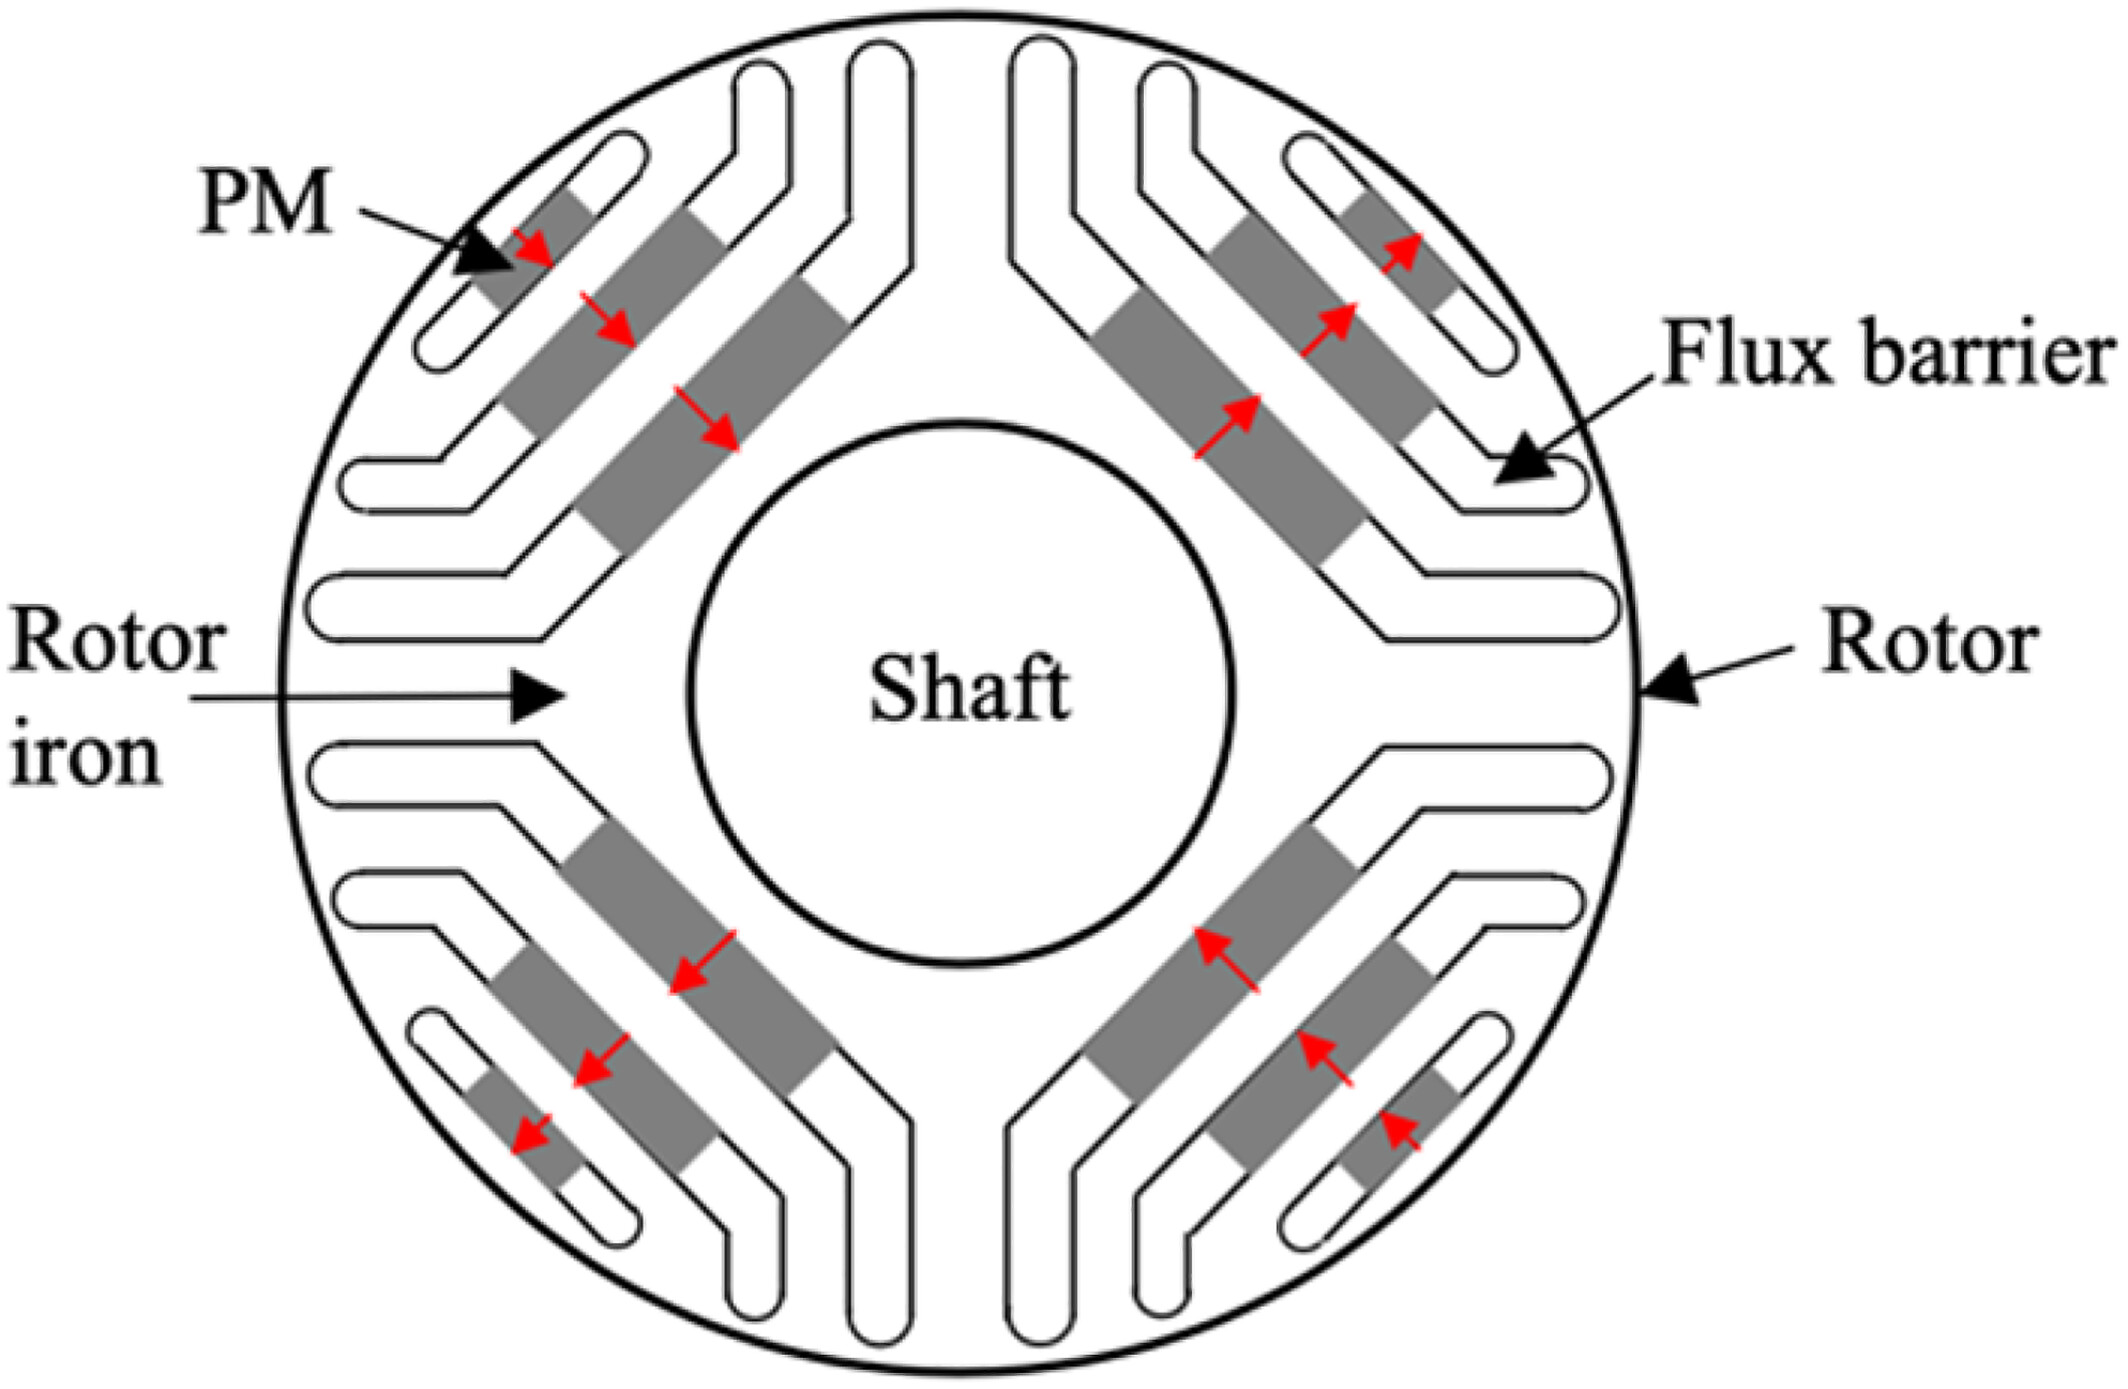
\includegraphics[width=0.5\textwidth]{src/png/pmsynrelm-rotor-magnets-q-axis.png}
            \caption{Rotor design of a Permanent Magnet Assisted Synchronous Reluctance Motor with permanent magnets oriented solely in the $q$-axis. \cite{tavernini-design-and-optimisation-of-energy-efficient-pmsynrelm-for-electric-vehicles}}
            \label{fig:pmsynrelm-rotor-magnets-q-axis}
    \end{figure}



    \subsection{Magnets}
        \gls{abbreviation:pmsynrelm} are very often compared to Permanent Magnet Synchronous Motors (\gls{abbreviation:pmsm}) used in the automotive field in terms of power and torque density, efficiency and costs. Though the \gls{abbreviation:pmsm} are very popular \cite{morimoto-experimental-evaulation-of-a-rare-earth-free-pmasynrm-with-ferrite-magnets-for-automotive-applications}, the \gls{abbreviation:pm}s used in their design often consist of rare-earth materials such as neodymium or dysprosium. That is the reason why \gls{abbreviation:pmsynrelm} motors with rare-earth-free materials are now being the subject of many research studies. Experiments comparing the production-used \gls{abbreviation:pmsm} and experimental prototype \gls{abbreviation:pmsynrelm} show, that the proposed prototype in \cite{mashiro-performance-of-mpasynrm-with-ferrite-magnets-for-ev-hv-applications-considering-productivity} achieve close values of power density and an efficiency as rare-earth \gls{abbreviation:pmsm} counterpart, but with much lower costs \cite{haiwei-low-cost-ferrite-pm-assisted-synchronous-reluctance-machine-for-electric-vehicles}.\par
It has been observed, that when inserting the \gls{abbreviation:pm} in the center of the flux barrier, a magnetic flux lines are forced to pass through the flex barriers in the $q$-axis. This results in the decreased linked magnetic flux in the $q$-axis and therefore improves the output torque. \cite{ibrahim-permanent-magnet-assisted-synchronous-reluctance-motor-employing-a-hybrid-star-delta-winding-for-high-speed-applicaitons, ngo-performance-analysis-of-synchronous-reluctance-motor-with-limited-amount-of-permanent-magnet} The two general types of rotor with embedded \gls{abbreviation:pm} are depicted in figure \ref{fig:pmsynrelm-rotor-magnets-position}.


    \begin{figure}[htbp!]
            \centering
            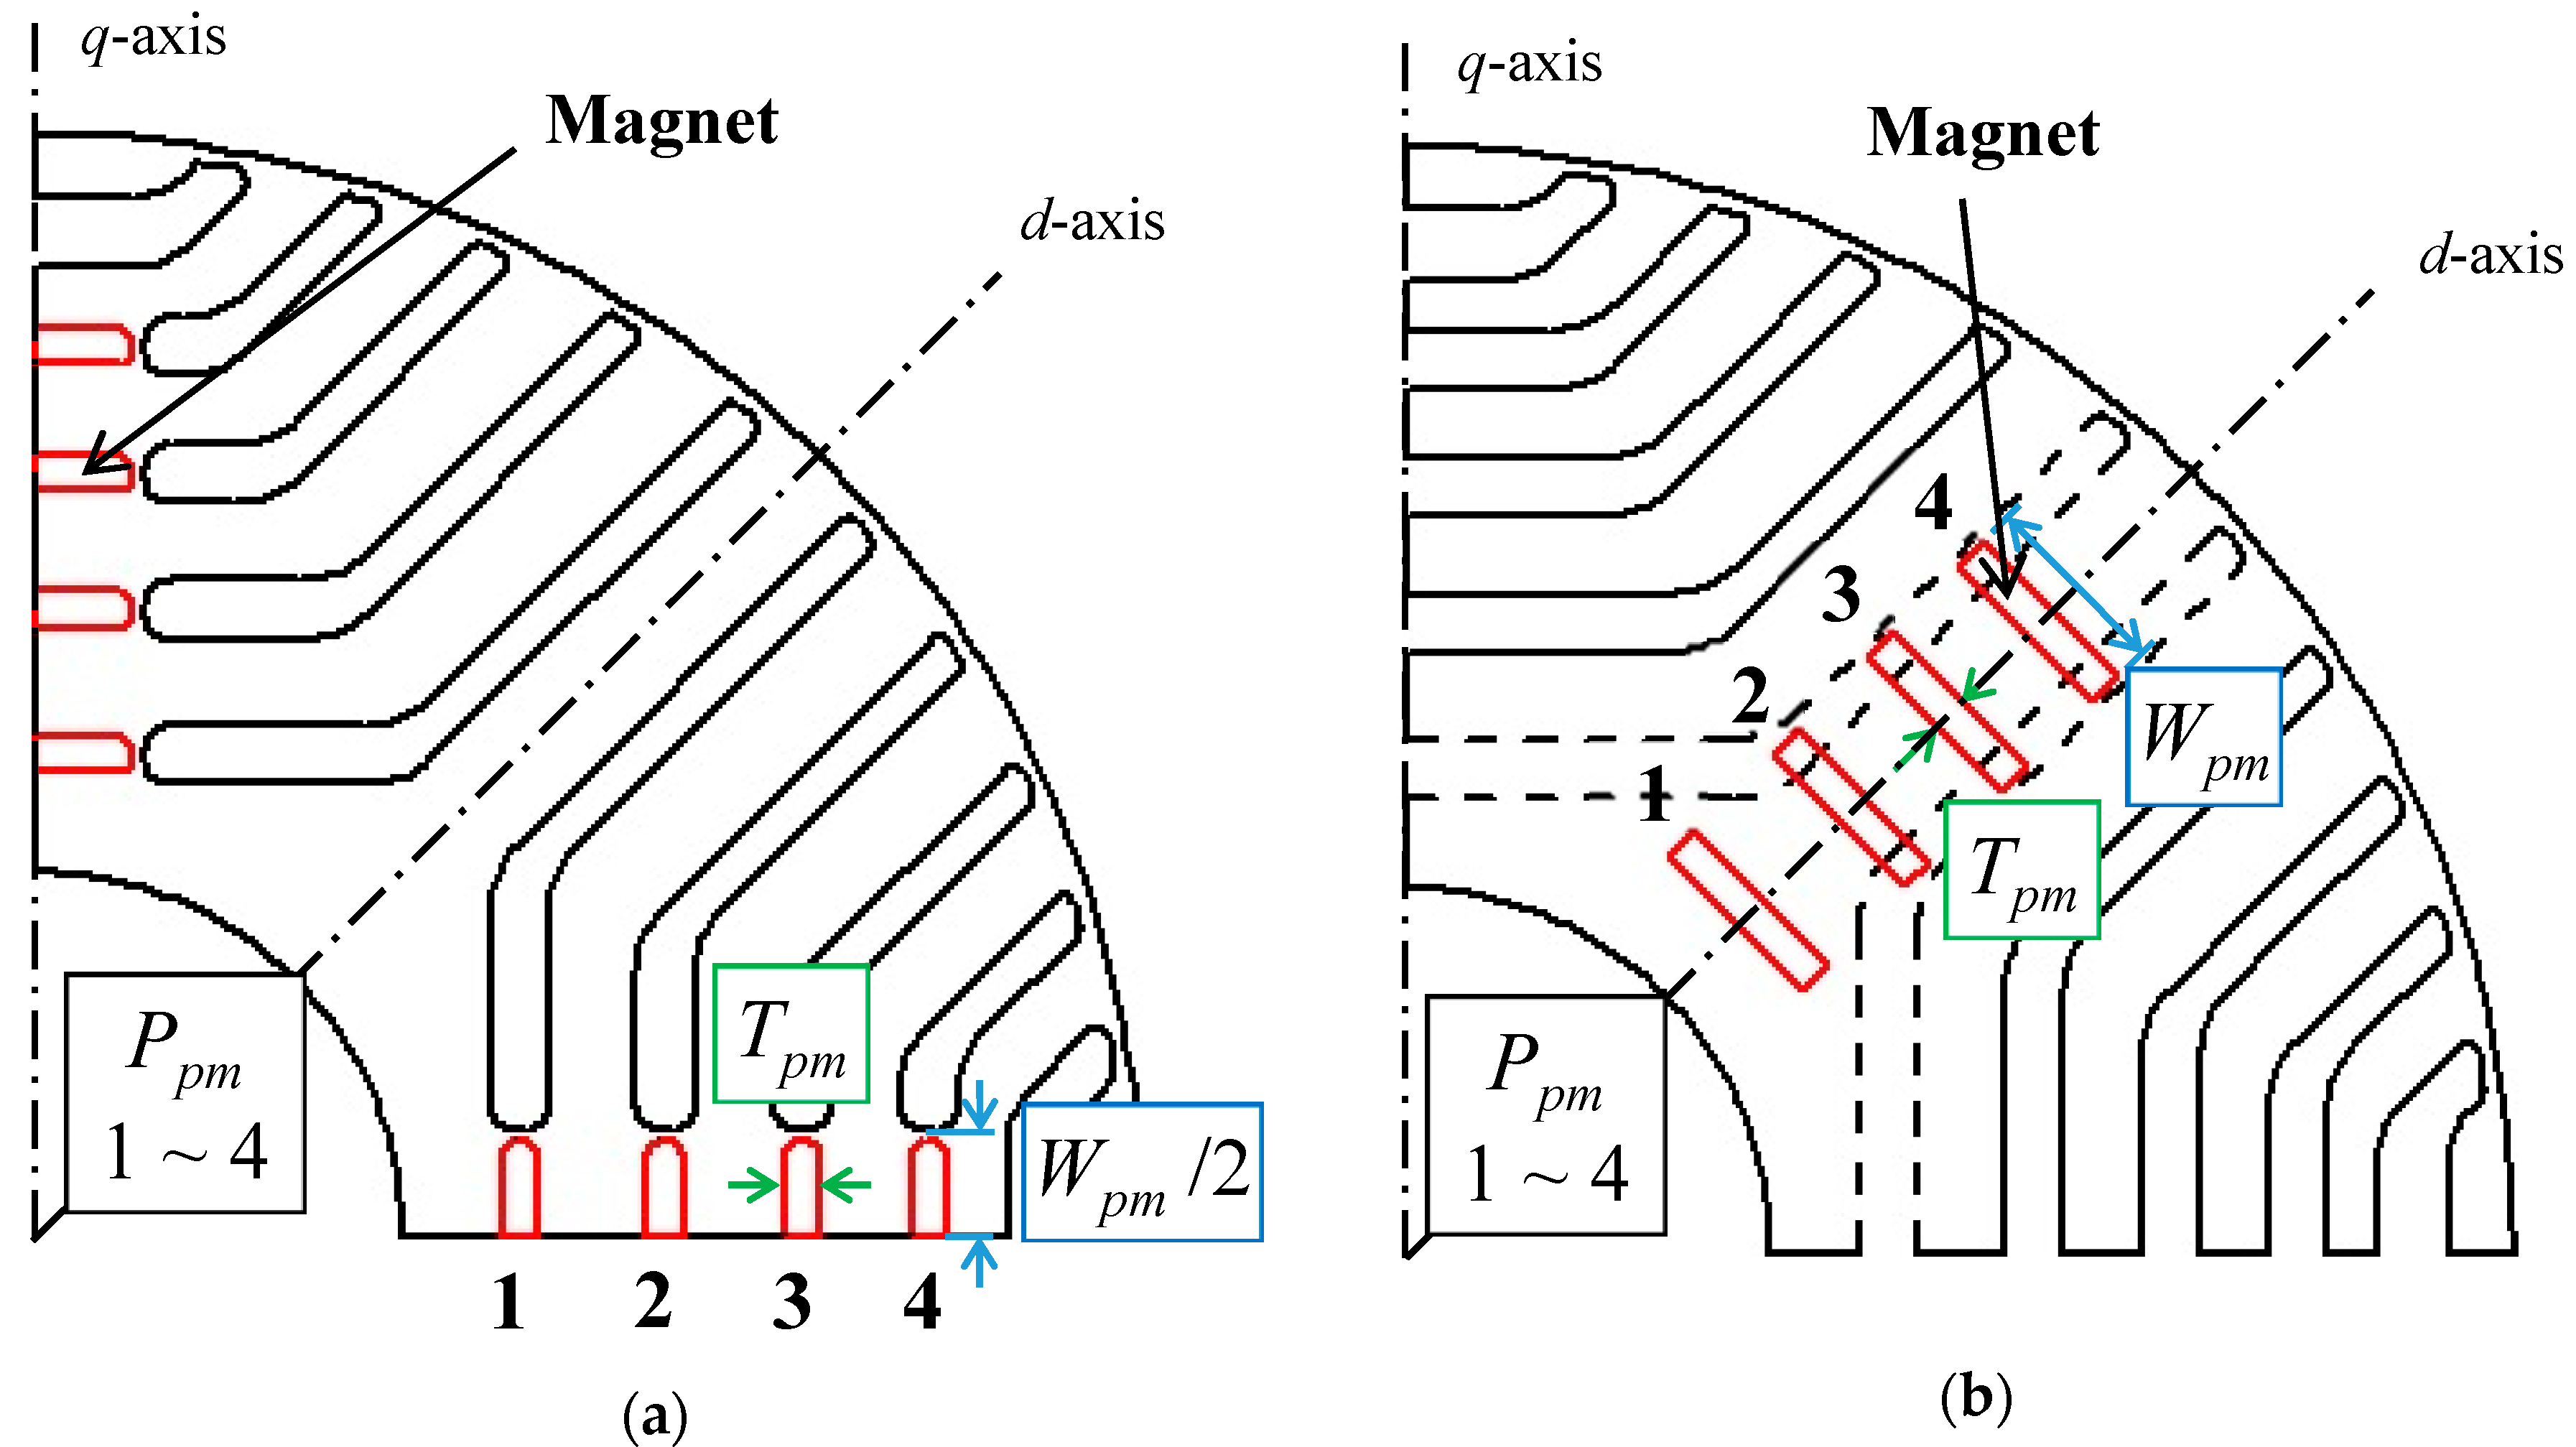
\includegraphics[width=0.8\textwidth]{src/png/pmsynrelm-rotor-magnets-position.png}
            \caption{Different approaches to permanent magnet orientation in the rotor of a Permanent Magnet Assisted Synchronous Reluctance Motor. (\textbf{a}) PM embedded along the flux bariers, facing the $q$-axis; (\textbf{b}) Permanent magnets are crossing the flux bariers, therefore facing the $d$-axis. \cite{ngo-performance-analysis-of-synchronous-reluctance-motor-with-limited-amount-of-permanent-magnet}}
            \label{fig:pmsynrelm-rotor-magnets-position}
    \end{figure}


\section{Control}

    \subsection{Mathematical model}
        The stator voltage equation of \gls{abbreviation:pmsynrelm} denoted in the general axis $k$ is as follows

        \begin{equation}
            \underline{u}^k_1 = \text{R}_\text{s} \underline{i}^k_1 + \frac{\dd \underline{\psi}^k_1 }{\dd t} + j \omega_k \underline{\psi}^k_1.
        \end{equation}

        Where $\underline{u}^k_1$ (V) is space vector of stator voltage, $R_\text{s}$ ($\Omega$) is stator rezistance, $\underline{i}^k_1$ (A) space vector of a stator current, $\underline{\psi}^k_1$ (Wb) space vector of a stator flux linkeage, $\omega_k$ (rad $\text{s}^{-1}$) general angular speed.\par
        The voltage equation denoted in $dq$-axis is as follows

        \begin{equation}
            \underline{u}^{dq}_1 = \text{R}_\text{s} \underline{i}^{dq}_1 + \frac{\dd \underline{\psi}^{dq}_1 }{\dd t} + j \omega_1 \underline{\psi}^k_1,
        \end{equation}
        
        where $\omega_1$ (rad $\text{s}^{-1}$) is electrical angular speed of a stator rotating magnetic field. When the equation is denoted in vector components and the subscript "1" for stator is omitted and the axis are newly denoted by the variables subscript

        \begin{equation}
            \underline{u}_d
        \end{equation}

    \subsection{Control strategies}

\section{Comparation to others}

\section{Usage}

%% Conclusion %%
\newpage
\addcontentsline{toc}{section}{\numberline{}Conclusion} 
\section*{Conclusion}

\flushbottom % vyčištění stránky

% konec závěru

\newpage
\setmonofont{Times New Roman}

%% REFERENCES %%
\printbibliography[title={{References}}]	
\nocite{*}
\setmonofont{CourierPrime-Regular}
\addcontentsline{toc}{section}{\numberline{}References} % Adding citations to TOC %

%% APPENDIX %%
\appendix
\titleformat{\section}{\color{ctublue}\fontspec{Times New Roman}\fontsize{15}{15}\bfseries}{Appendix \thesection:}{2.1em}{}

\begin{appendices}
	\section{List of symbols and abbreviations}

		\printglossary[type=abbreviationslist, style = myStyleAbbreviations]

		\fbar
		%\newpage
		\printglossary[type=symbolslist, style =  myStyleSymbols]

	\end{appendices}
\end{document}
